\chapter{Contend of the DVD}
\begin{itemize}
	\item \textbf{thesis.pdf} - PDF version of the thesis text.
	\item \textbf{tex/} - \LaTeX ~source codes of the thesis text.
	\item \textbf{src/} - Source codes of our program described in chapter~\ref{chapter:implementation}.
	\item \textbf{datasets/} - Collected image datasets described in the section~\ref{sec:experiments-datasets} and some other.
	\item \textbf{experiments/} - Experimental results used in chapter~\ref{chapter:experiments}.
	\item \textbf{third\textunderscore party/} - Other Structure from Motion and Bundle Adjustment application sources.
	\item \textbf{samples/} (works only if whole content of the DVD is copied to a local directory)
	\begin{itemize}
		\item \textbf{calibrated\textunderscore ordered/} - Runs predefined scenario with known intrinsic camera parameters on ordered image collection.
		\item \textbf{calibrated\textunderscore unordered/} - Runs predefined scenario with known intrinsic camera parameters on unordered image collection.
		\item \textbf{calibrated\textunderscore custom/} - Runs structure from motion on a custom dataset (images must be in folder \texttt{dataset}) from one camera where the calibration pictures of checker board must be provided in folder \texttt{calibration}.
		\item \textbf{uncalibrated/} - Runs predefined scenario with unknown camera calibration on unordered image collection.
		\item \textbf{uncalibrated\textunderscore custom/} - Runs the program on a custom dataset (on images in folder \texttt{dataset}) with unknown calibration.
	\end{itemize}
	\item \textbf{install.sh} - Installation script (requires OpenCV and cmake to be installed).
	\item \textbf{bin/} - Location of a binary version of the program after running \texttt{install.sh}.
\end{itemize}
\chapter{Poster}
\begin{figure}[h]
	\begin{center}
		\includegraphics[keepaspectratio,width=10cm]{fig/poster.pdf}
	\end{center}
	\caption{Preview of poster presenting our program.}
	\label{fig:posteri}
\end{figure}
\chapter{Installation and Sparse Reconstruction}
\chapter{Dense Reconstruction with VisualSFM}
\label{visualsfm:reconstruction}
The VisualSFM is an amazing collection of software that can create dense reconstruction from random images of a static scene. The application has a graphical user interface depicted in figure~\ref{fig:visualsfm-gui}.
\begin{figure}[h]
	\begin{center}
		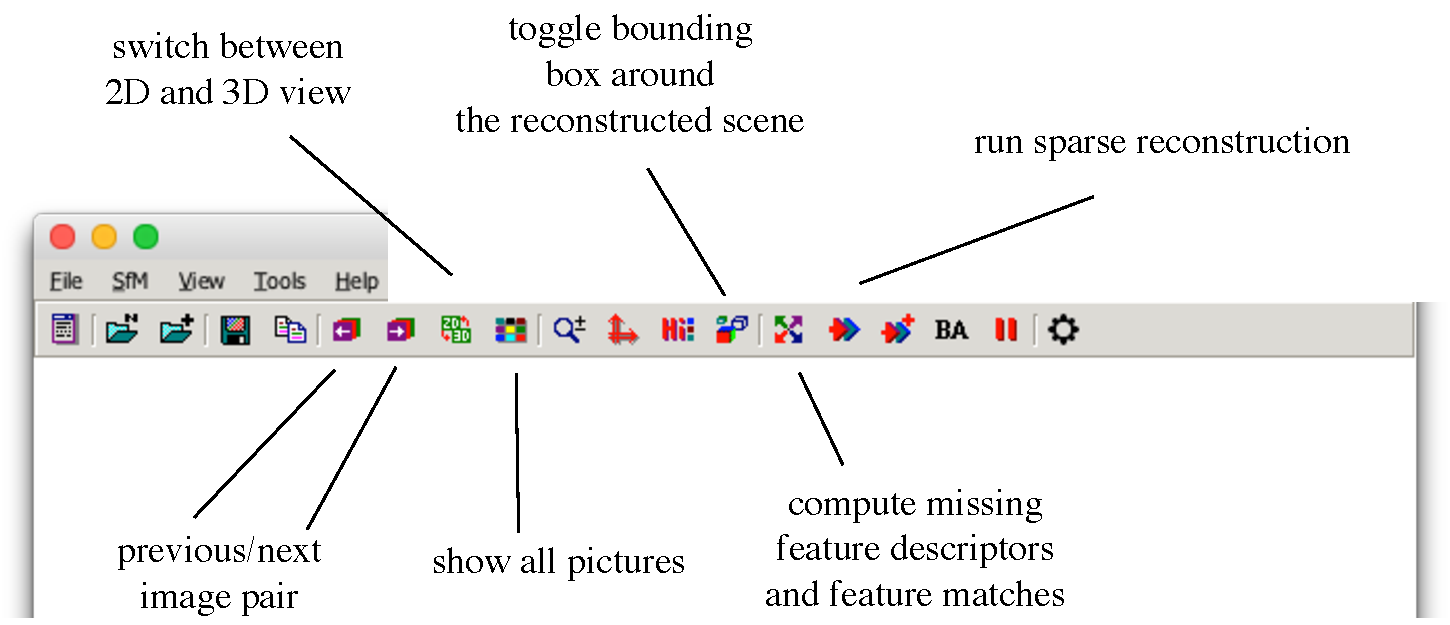
\includegraphics[keepaspectratio,width=\textwidth]{fig/visualsfm-gui.pdf}
	\end{center}
	\caption{GUI of the VisualSFM with few important buttons.}
	\label{fig:visualsfm-gui}
\end{figure}
\section{Reconstruction Process}
The whole process of reconstruction follows:
\begin{itemize}
	\item[1.] Choose \textbf{File} $\rightarrow$ \textbf{Open+ Multi Images}, navigate yourself to the dataset and select desired photos. After a while the photos should load into the system and should be displayed in a matrix.
	\item[2.] Next we need to compute keypoints and feature correspondences. Click 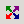
\includegraphics[keepaspectratio,width=.5cm]{fig/visualsfm-compute-matches.png} or choose \textbf{SfM} $\rightarrow$ \textbf{Pairwise Matching} $\rightarrow$ \textbf{Compute Missing Match}. The system will now detect keypoints and calculate matches for all new photos. These feature and matches are implicitly cached in separate files \texttt{.sift} and \texttt{.mat}. Please note that this step may take a significant amount of time. The progress is shows in the \textbf{Log Window}.
	\item[3.] Click on the button 
\includegraphics[keepaspectratio,width=.5cm]{fig/visualsfm-sparse-reconstruction.png} or choose \textbf{SfM} $\rightarrow$ \textbf{Reconstruct Sparse} to compute sparse reconstruction. The view should change slightly showing the reconstructed 3D scene. The program may not create single model for the input dataset, but you can browse distinct models by pressing up and down arrow keys (model number is indicated in the window name between first pair of square brackets).
	\item[4.] Last step is running the dense reconstruction. Click 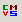
\includegraphics[keepaspectratio,width=.5cm]{fig/visualsfm-dense-reconstruction.png} or choose \textbf{SfM} $\rightarrow$ \textbf{Reconstruct Dense}. You will be prompted to choose working directory and once all the files are saved to this directory, the PMVS2 dense reconstruction starts. Note that the dense reconstruction is a complex problem and takes a lot of time. Once finished, you can toggle between sparse and dense with hotkey \textbf{tabulator}. An example of sparse and dense reconstruction is in the figure~\ref{fig:visualsfm-sparse-dense}.
\end{itemize}
The output, dense structure of each model is stored in folder \texttt{models} in a PLY format. The estimated camera calibrations can be found in the text file \texttt{cameras\textunderscore v2.txt}. The camera centres are stored in the PLY format as  \texttt{centers-[model\textunderscore ID].ply} containing the 3D locations for every camera in each model.
\begin{figure}[h]
	\begin{center}
		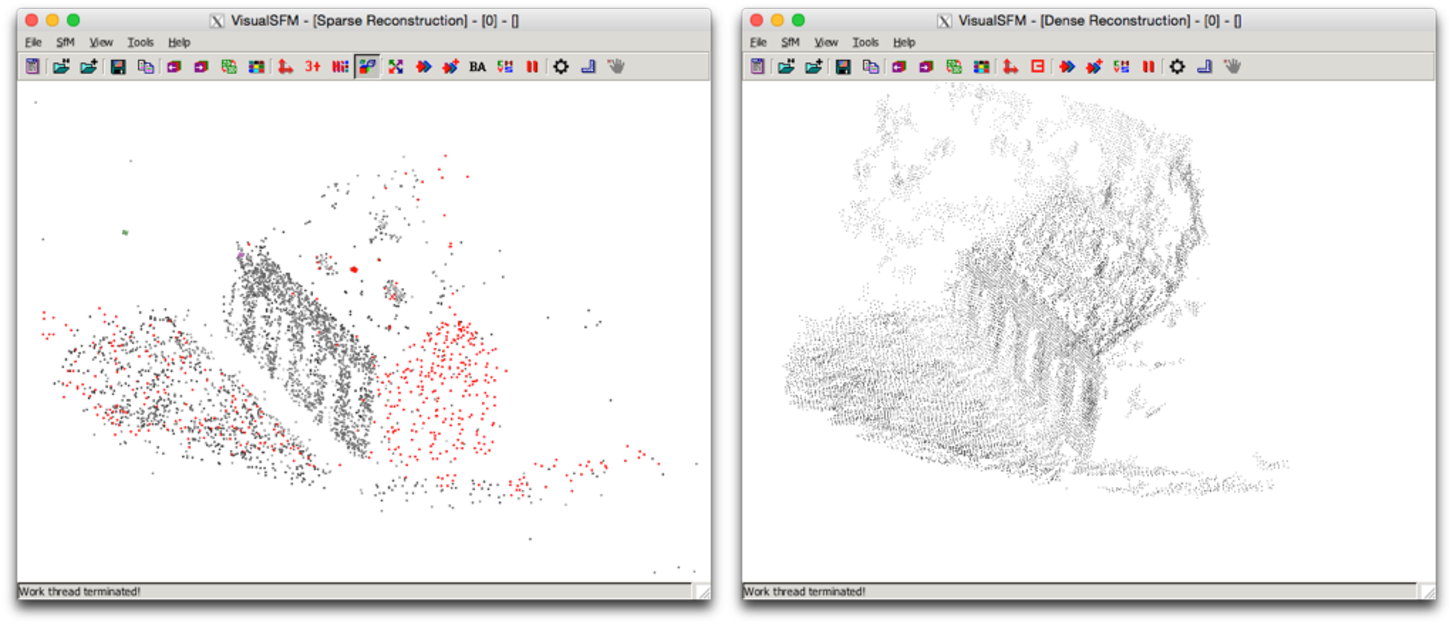
\includegraphics[keepaspectratio,width=\textwidth]{fig/visualsfm-sparse-dense.pdf}
	\end{center}
	\caption{Sparse (left) and dense (right) reconstruction of the Model House dataset.}
	\label{fig:visualsfm-sparse-dense}
\end{figure}

\section{Useful Tips and Controls}
The VisualSFM offers many hidden functionality useful for reconstructing the 3D scene. Full list can be found in the VisualSfM online documentation\footnote{VisualSfM documentation \url{http://ccwu.me/vsfm/doc.html}}.
\begin{itemize}
	\item \textbf{Camera calibration.} If camera calibration is known, it can be provided to the program by choosing \textbf{SfM} $\rightarrow$ \textbf{More Functions} $\rightarrow$ \textbf{Set Fixed Calibration}. This calibration can be also made shared across all cameras.
	
	\item \textbf{Selecting Initial Pair.} Initial camera pair for the reconstruction can be chosen by selecting the pair with left and right arrow keys and then choosing \textbf{SfM} $\rightarrow$ \textbf{More Functions} $\rightarrow$ \textbf{Set Initialization Pair}.
	
	\item \textbf{Keyboard shortcuts and mouse controls.}
	
	\begin{tabular}{l l}
		\textbf{Mouse middle wheel} & Zoom the scene. \\
		\textbf{Right mouse drag} & Rotate the scene. \\
		\textbf{Left mouse drag} & Pan the scene. \\
		\textbf{Tabulator} & Switch between sparse and dense reconstruction. \\
		\textbf{Up/Down} & Switch between different models. \\
		\textbf{Left/Right} & Switch between camera pairs. \\
		\textbf{T} & Switch between visualization modes: \begin{tabular}{l}
			\text{1) cameras + 3D points} \\
			\text{2) cameras only} \\
			\text{3) 3D points only} \\
		\end{tabular}\\
	\end{tabular}
\end{itemize}

\chapter{Dense to Textured Surface Reconstruction using Meshlab and Blender}
\label{app:surface-reconstruction}
This chapter describes the process of creation textured 3D polygonal model from dense point cloud. It assume that the user have a 3D dense reconstruction in a format produced by VisualSFM. The process start in MeshLab:
\begin{itemize}
	\item[1.] In MeshLab, select \textbf{File} $\rightarrow$ \textbf{OpenProject} and choose file \texttt{bundle.rd.out} in the dense reconstruction data folder. Next prompt requires the \texttt{list.txt} from the same folder. 
	\item[2.] Right now the sparse point cloud is opened which is not what we want. Click the icon 
\includegraphics[keepaspectratio,width=.5cm]{fig/meshlab-layers.png} or \textbf{View} $\rightarrow$ \textbf{Show Layer Dialog}. A new toolbar will appear on the right of the screen. Click on the model with the right mouse button and from the context menu select \textbf{Delete Current Mesh} (as depicted in figure~\ref{fig:meshlab-1}).
\begin{figure}[h]
	\begin{center}
		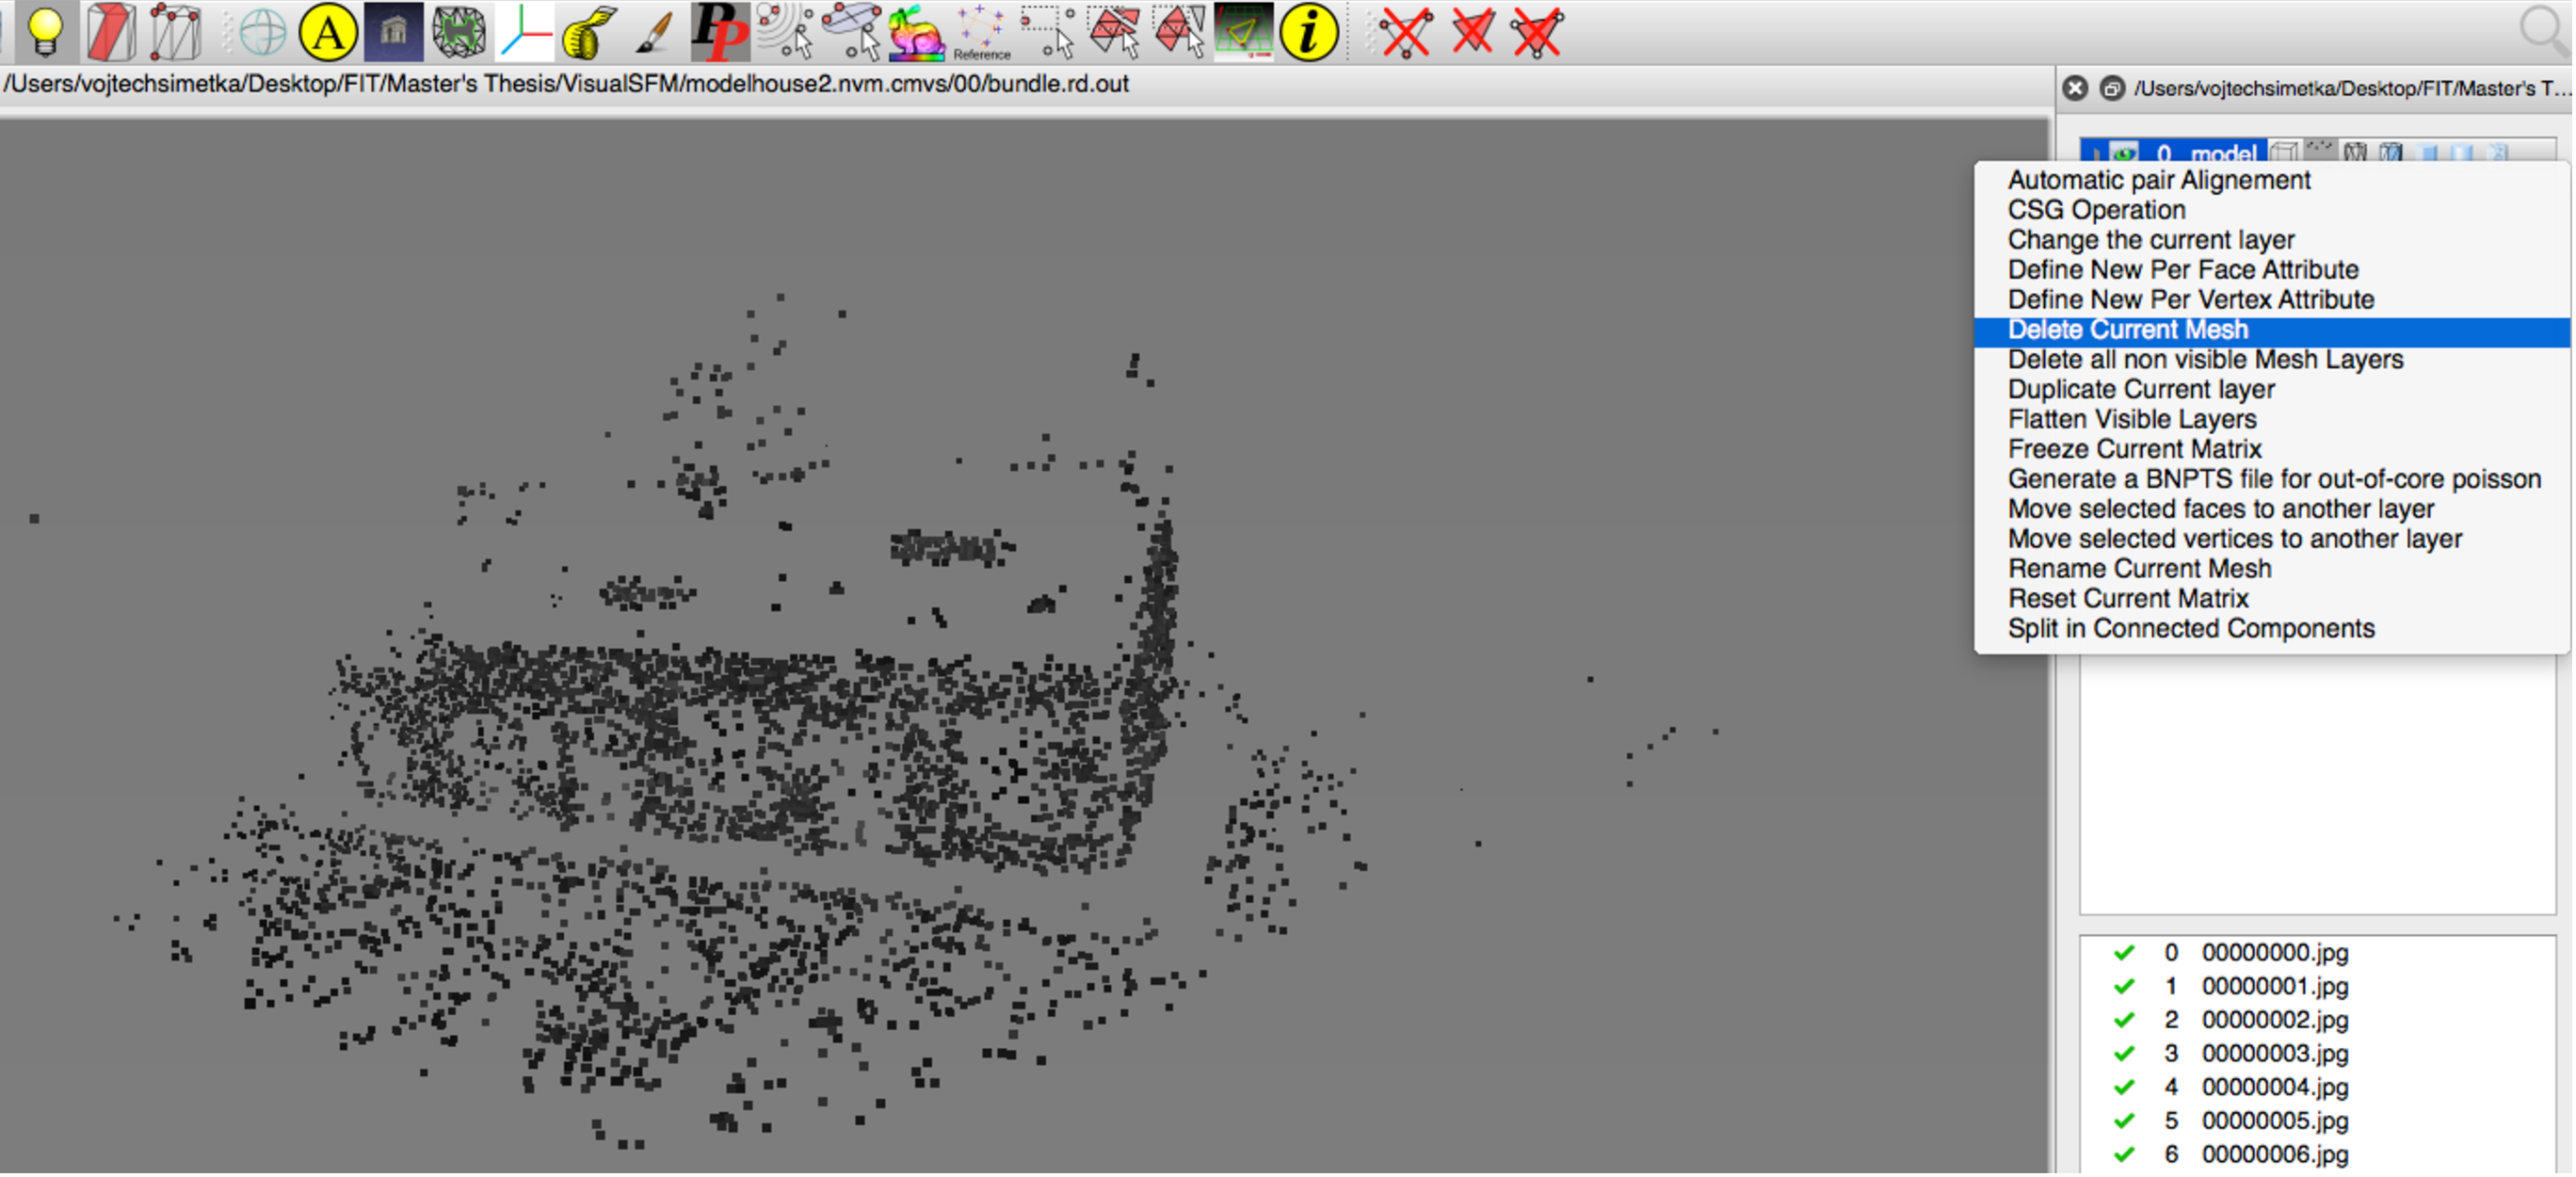
\includegraphics[keepaspectratio,width=9cm]{fig/meshlab-1.pdf}
	\end{center}
	\caption{How to erase sparse cloud mesh in MeshLab.}
	\label{fig:meshlab-1}
\end{figure}
	\item[3.] Choose \textbf{File} $\rightarrow$ \textbf{Import Mesh} and select adequate model from folder \texttt{models}.
	\item[4.] The model shown is now a dense point cloud, but it is almost certainly quite noisy. We can remove some of the noisy data by selecting them with tool 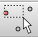
\includegraphics[keepaspectratio,width=.5cm]{fig/meshlab-select.png} (\textbf{Edit} $\rightarrow$ \textbf{Select Vertices}), and erasing them with 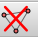
\includegraphics[keepaspectratio,width=.5cm]{fig/meshlab-delete.png}.

	\item[5.] Next step is to create a surface reconstruction. Choose \textbf{Filters} $\rightarrow$ \textbf{Point Set} $\rightarrow$ \textbf{Surface Reconstruction: Poisson}. We suggest you to use following values:
	
	\begin{tabular}{l l}
		Octree Depth & 12 \\
		Solver Divide & 10 \\
		Samples per Node & 1 \\
		Surface offsetting & 1 \\
	\end{tabular}
	
%\begin{figure}[ht]
%	\begin{center}
%		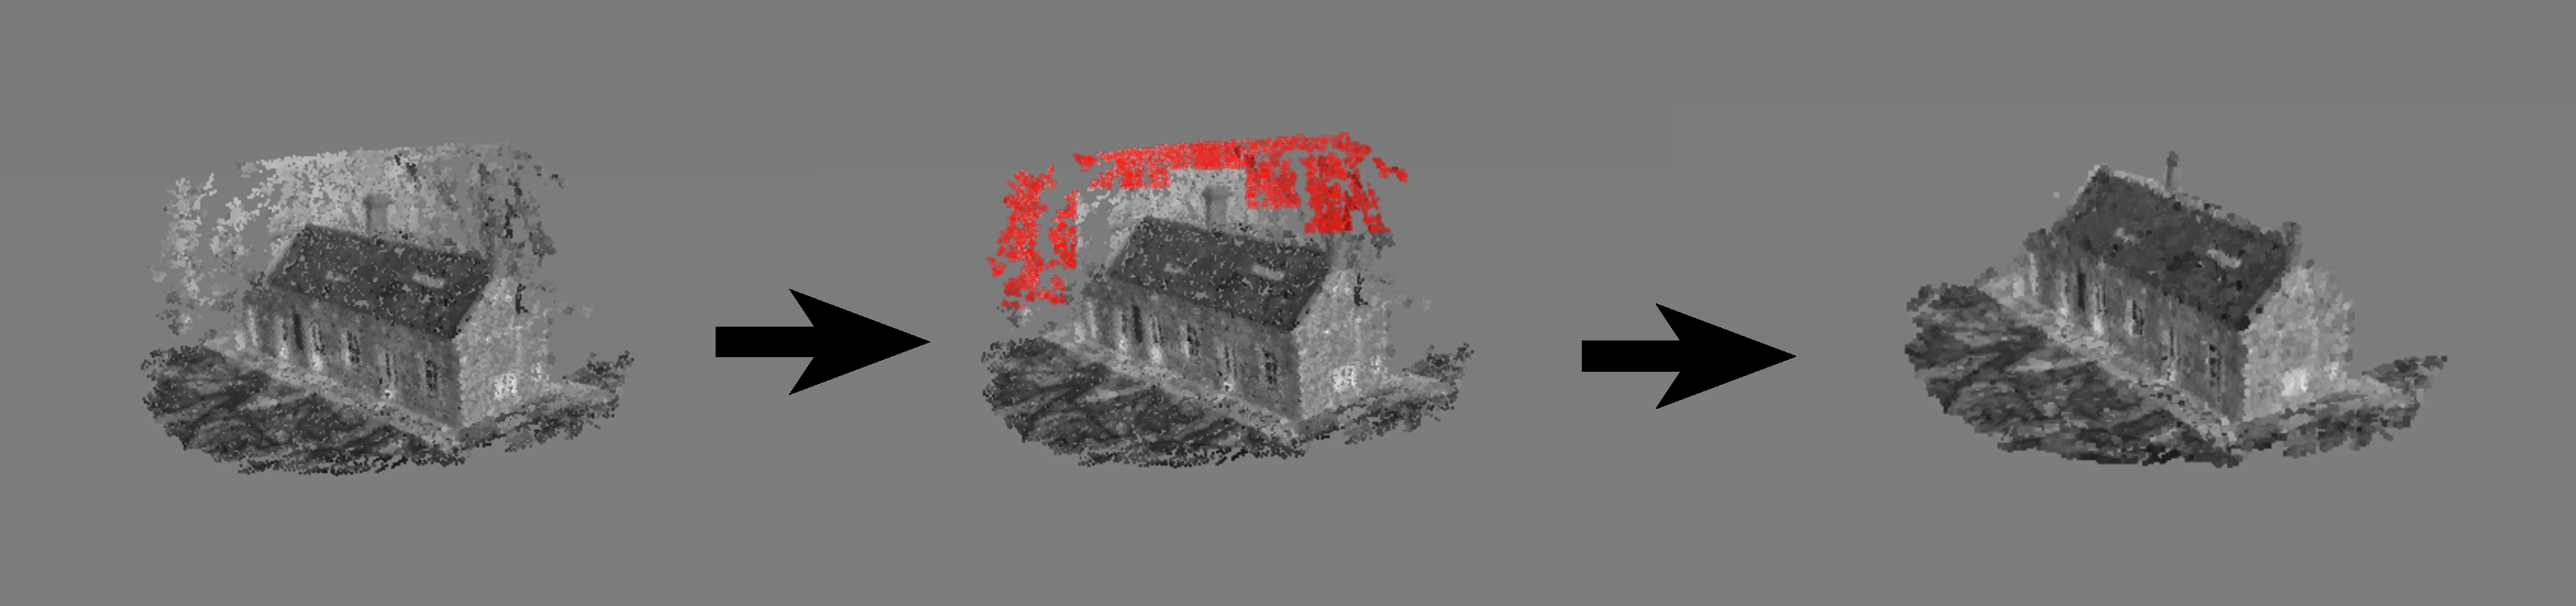
\includegraphics[keepaspectratio,width=\textwidth]{fig/meshlab-2.pdf}
%	\end{center}
%	\caption{The process of manually erasing incorrect points.}
%	\label{fig:meshlab-2}
%\end{figure}

	\item[6.] However, the surface reconstruction creates a lots of incorrect faces. We once again erase the vertices using tools from step 4. Once done, choose \textbf{Filters} $\rightarrow$ \textbf{Selection} $\rightarrow$ \textbf{Select non-manifold Edges}, hit apply and erase these points with vertex erase tool 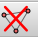
\includegraphics[keepaspectratio,width=.5cm]{fig/meshlab-delete.png}.
	
	\item[7.] Now we finally apply textures. Select \textbf{Filters} $\rightarrow$ \textbf{Texture} $\rightarrow$ \textbf{Parametrization + texturing from registered rasters}. Make sure the following options are checked: \textbf{Color correction, Use distance weight, Use image border weight, Clean isolated triangles} and \textbf{UV stretching}.
	\item[8.] The last step in the MeshLab tool is to export the model to the file format supported by Blender. Select \textbf{File} $\rightarrow$ \textbf{Export mesh as} and make sure you save it as an \texttt{obj} type.
\end{itemize}

The next part is more or less optional and contains mostly just storing the texture in the file itself.
\begin{itemize}
	\item[1.] Lets open Blender, right click on the cube, hit key \textbf{x} and click delete.
	\item[2.] Choose \textbf{File} $\rightarrow$ \textbf{Import} $\rightarrow$ \textbf{Wavefront (.obj)}.
	\item[3.] On the panel on the right select texture tab. Add new texture and change the type of the texture to \textbf{Image or Movie}. Ten press \textbf{Open} and load the appropriate texture file. If necessary the UV mapping coordinates can be altered, but this is beyond the scope of our tutorial.
	\item[4.] Now we can export the 3D model to some reasonable 3D file format, for example the\texttt{fbx}.
\end{itemize} 


\begin{figure}[ht]
	\begin{center}
		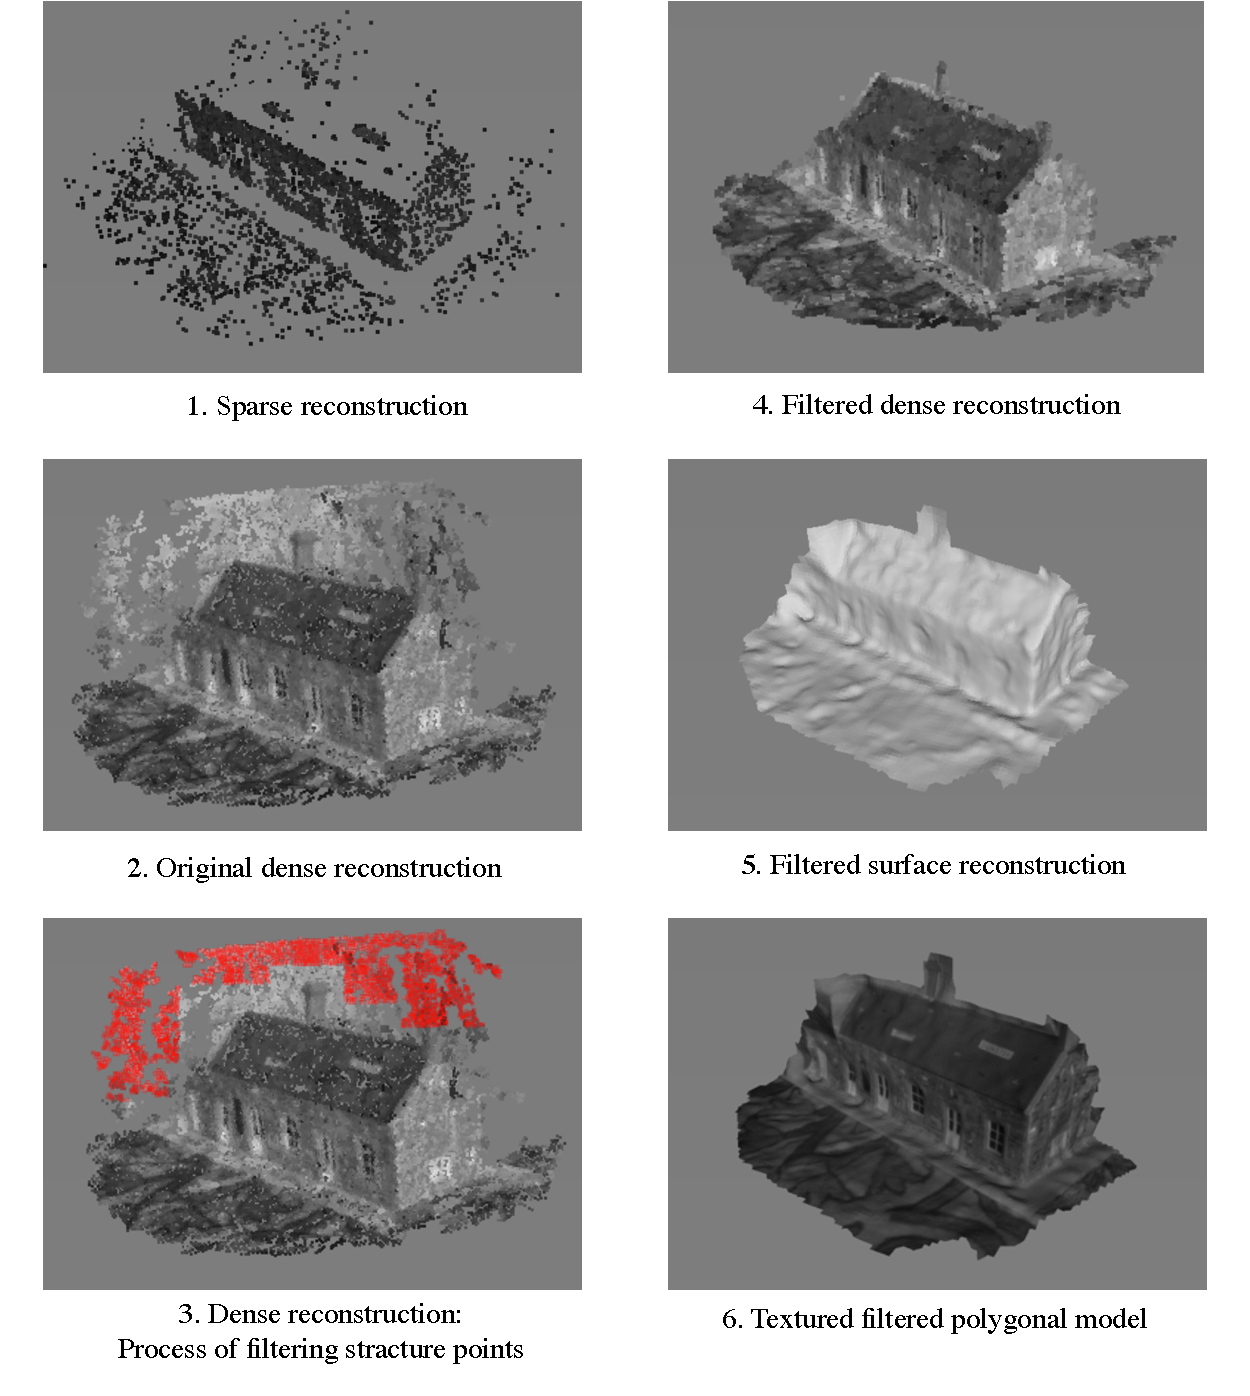
\includegraphics[keepaspectratio,width=\textwidth]{fig/reconstruction-overview.pdf}
	\end{center}
	\caption{Distinct reconstruction phases from sparse reconstruction to textured 3D model.}
	\label{fig:reconstruction-overview}
\end{figure}

%\chapter{Manual}
%\chapter{Konfigrační soubor}
%\chapter{RelaxNG Schéma konfiguračního soboru}
%\chapter{Plakat}
